\documentclass[
coverheight=9in,
coverwidth=6in,
spinewidth=0.468in,
bleedwidth=.125in,%.125in,
marklength=0in,
markcolor=black]{bookcover}

\usepackage[T1]{fontenc}

\newbookcoverpart{pfront}{
\setpartposx{\marklength+\bleedwidth+\spinewidth+\coverwidth+6mm}
\setpartposy{\marklength+\bleedwidth+5mm}\setpartheight{\coverheight-5mm}
\setpartwidth{\coverwidth-13mm}
\settrimmedpart{0mm}{0mm}{0pt}{0pt}
}

\newbookcoverpart{pback}{
\setpartposx{\marklength+\bleedwidth+6mm}
\setpartposy{\marklength+\bleedwidth+6mm}\setpartheight{\coverheight-12mm}
\setpartwidth{\coverwidth-12mm}
\settrimmedpart{0mm}{0mm}{0pt}{0pt}
}

\begin{document}

\begin{bookcover}

\definecolor{mycolor}{HTML}{89bace}
\bookcovercomponent{color}{bg whole}{mycolor}

\definecolor{textcolor}{HTML}{0b4d66}

\bookcovercomponent{center}{front}{
\vskip-.1in
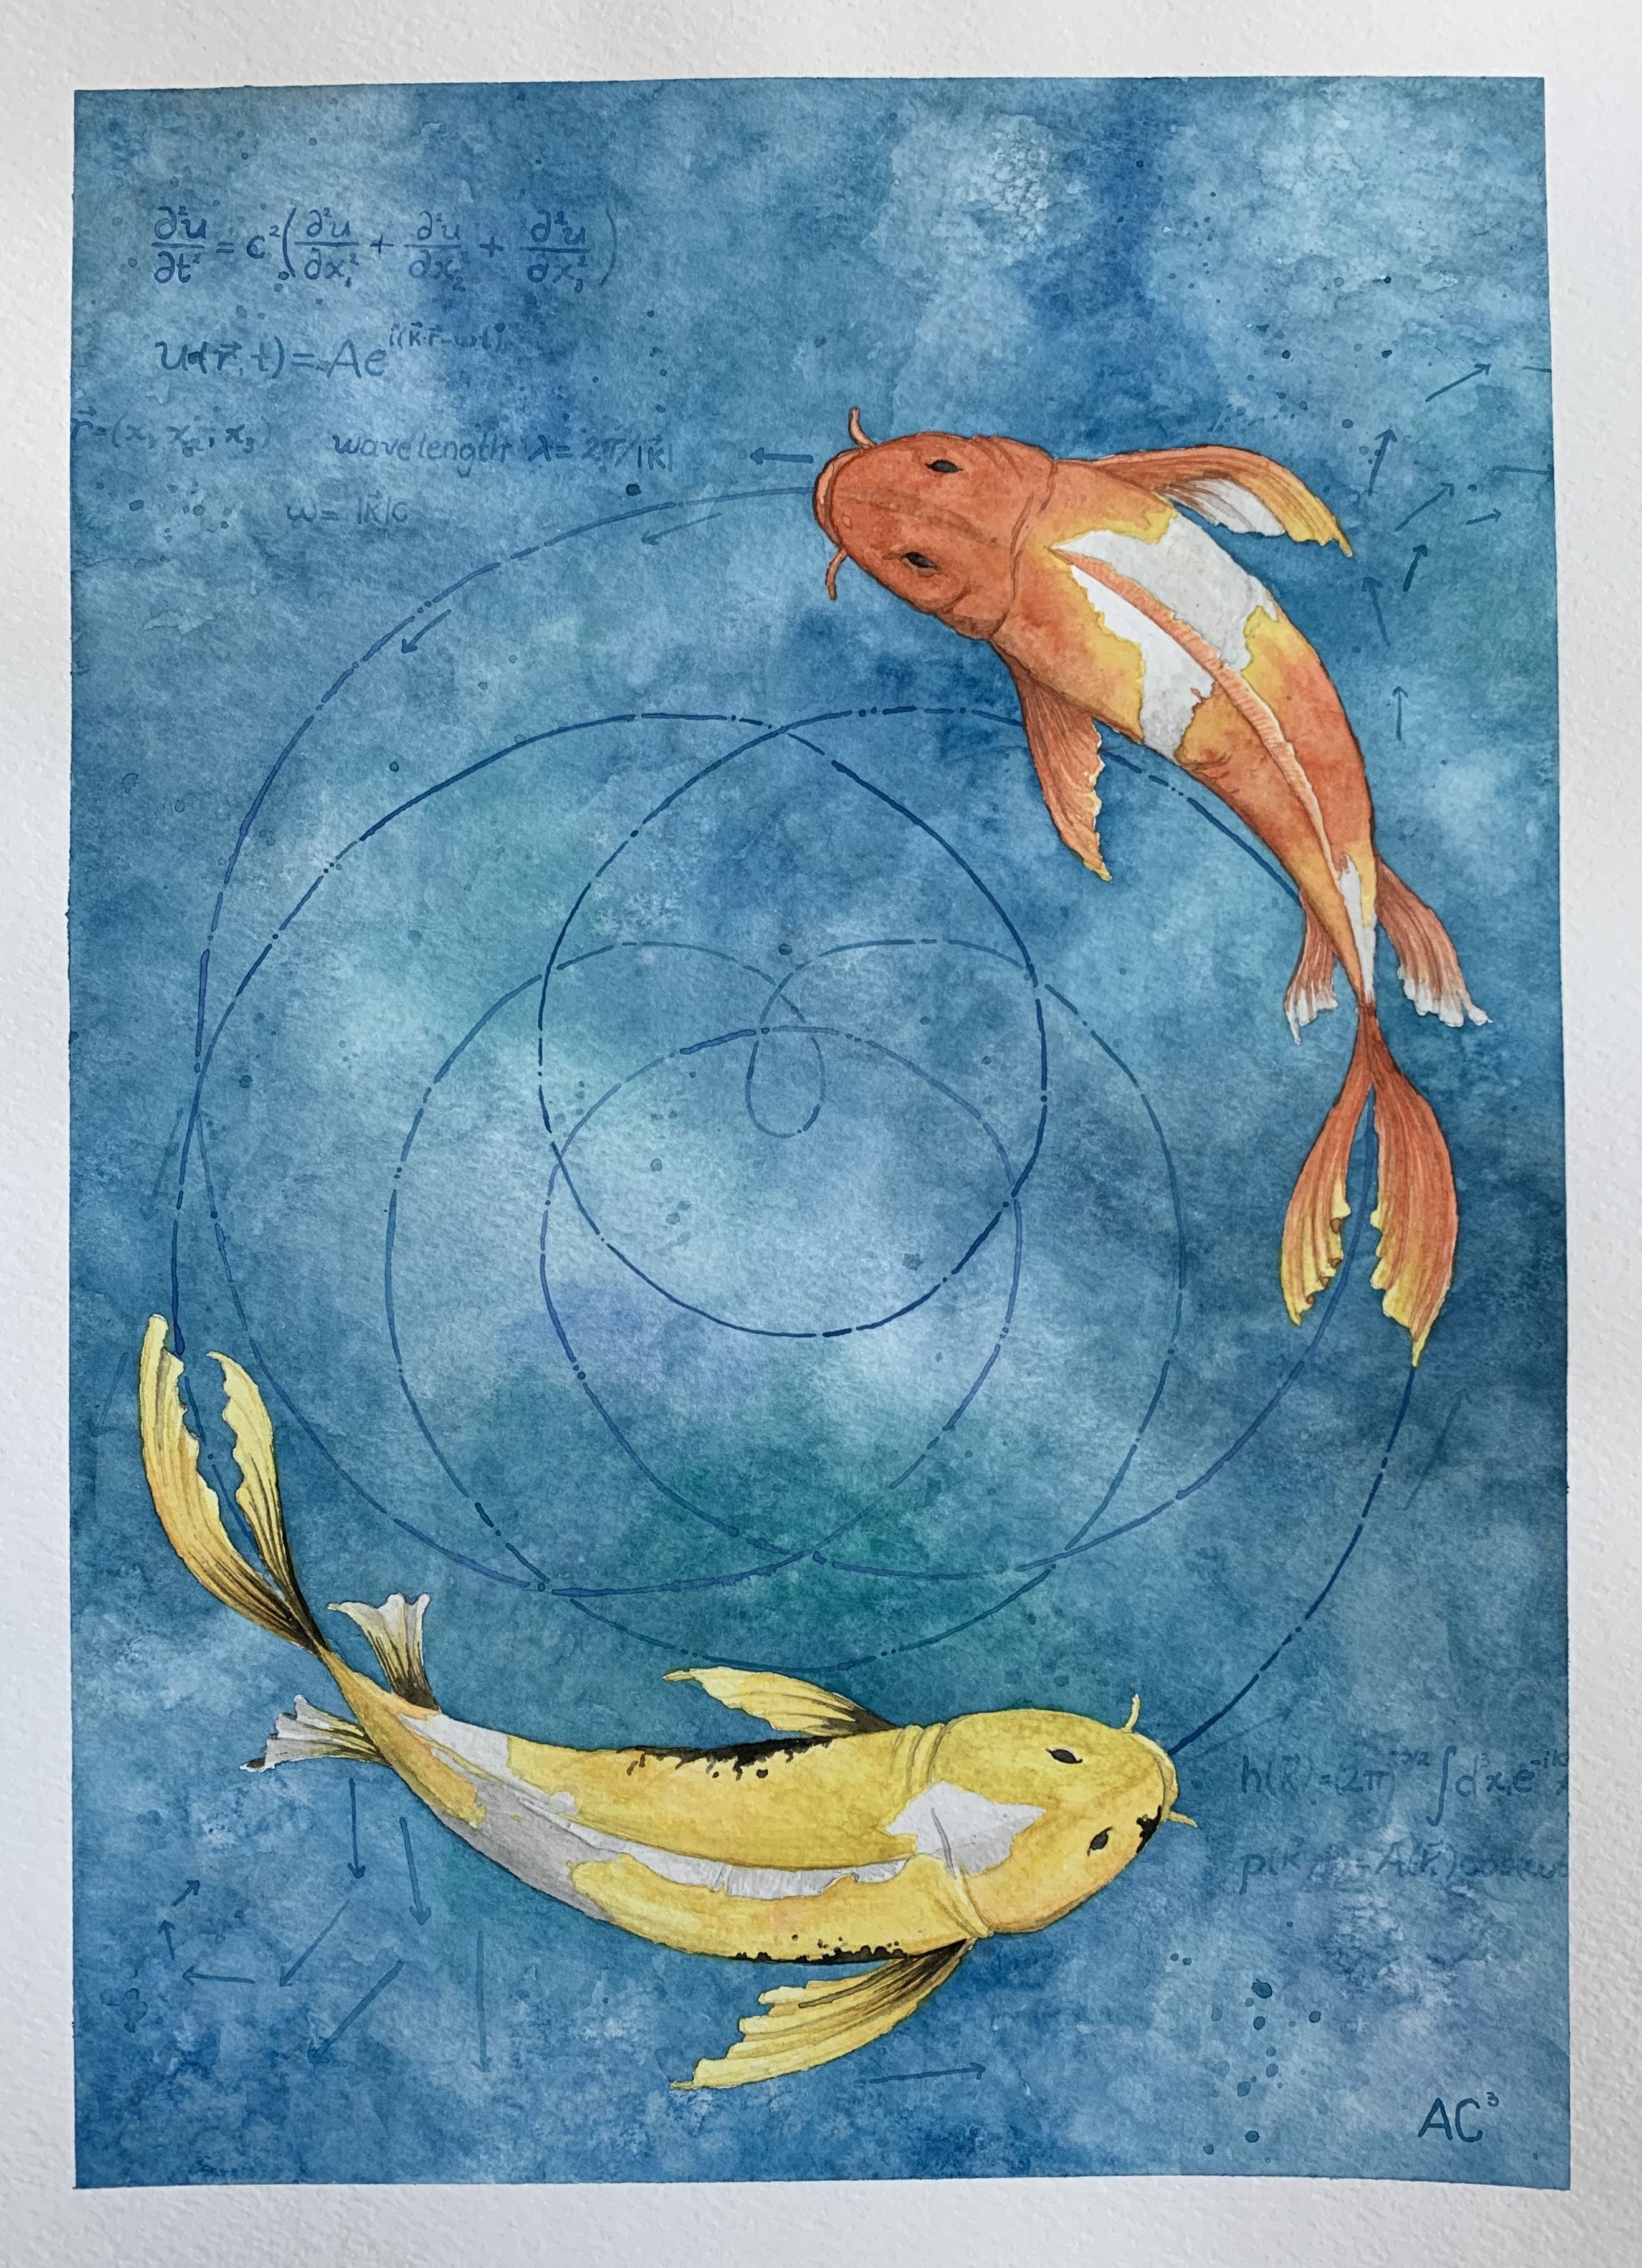
\includegraphics[trim=125 145 155 145, clip,width=\textwidth]{fish}
\vfill
}

\bookcovercomponent{center}{spine}
{\rotatebox[origin=c]{-90}{
\color{textcolor}
\fontsize{18}{25}\usefont{OT1}{lmtt}{b}{n}
       WHAT IS DIFFERENTIAL GEOMETRY: CURVES AND SURFACES}}

\bookcovercomponent{center}{pfront}{
\begin{center}
{\color{white}\fontsize{24}{28}\usefont{OT1}{lmtt}{b}{n}
WHAT IS DIFFERENTIAL GEOMETRY\\[5mm]
}
{\color{white}{\color{white}\fontsize{37}{28}\usefont{OT1}{lmtt}{b}{n}CURVES AND SURFACES}\hskip-1mm
}
\end{center}
\vfill
\begin{center}
{\color{textcolor}\ttfamily\LARGE{Anton Petrunin and
Sergio Zamora Barrera}
}
\end{center}
}

\bookcovercomponent{center}{pback}{
\begin{flushleft}
\parbox{.8\textwidth}{
\ttfamily\large\color{textcolor}
Please send all misprints, comments, suggestions to \texttt{petrunin@math.psu.edu}}
\end{flushleft}
\vfill
\begin{flushleft}
{\color{textcolor}\ttfamily\large github.com/anton-petrunin/gauss}
\end{flushleft}
}
\end{bookcover}

\end{document}
